\documentclass[12pt]{article}
\usepackage[a4paper,margin=1in]{geometry}
\usepackage{amsmath, amssymb}
\usepackage{graphicx}
\usepackage{booktabs}
\usepackage{hyperref}
\usepackage{algorithm}
\usepackage{algorithmic}
\usepackage{caption}
\usepackage{natbib}

\title{An Integer Programming Approach to Solving Rummikub Configurations}
\author{M. Zermeño \\ School of Physics and Mathematics \\ UANL}
\date{\today}

\begin{document}

\sloppy
\maketitle

\begin{abstract}
\sloppy
Rummikub is a popular tile-based game that involves both combinatorial optimization 
and strategic decision-making. This paper presents a formal investigation into the game 
mechanics, identifies the core computational challenges, and introduces an integer 
programming (IP) model designed to find optimal moves for a given player state. 
We analyze the problem space, define constraints based on legal game rules, and 
propose an IP formulation to maximize score per turn. Giving a future insight into 
applying possible Counting strategies to optimize decision making when given 
multiple players' states.
\end{abstract}

\section{Introduction}
Rummikub is a widely played tile-based game that combines elements of rummy and mahjong. 
Players aim to be the first to empty their racks by forming sets and runs using numbered 
and colored tiles. While the rules are simple, the combinatorial complexity that emerges 
as the game progresses makes decision-making increasingly difficult. A player may have 
many possible ways to arrange their tiles on the board, particularly when they are allowed 
to manipulate existing sets. Deciding on the best possible move—i.e., the one that maximizes 
the number or value of tiles placed on the table—is a non-trivial problem.

In this research, we investigate the use of Integer Linear Programming (ILP) to solve the 
Rummikub move optimization problem. Our goal is to develop a mathematical model that, given 
a current board state and a player's hand, determines the optimal set of tile moves that 
obey all Rummikub rules while maximizing a strategic objective, such as the number or 
value of tiles placed. This approach is based on the successful work of Den Hertog and 
Hulshof (2006), who showed that Rummikub configurations can be effectively modeled and 
solved using ILP within seconds, even in nontrivial game states.

\subsection{Why use Integer Linear Programming?}
Integer Linear Programming is a branch of mathematical optimization used for solving decision
problems involving discrete variables and linear relationships. In ILP, the goal is to 
maximize or minimize a linear objective function (like total tile value placed), subject 
to a set of linear equality or inequality constraints (like the legal formation of sets).

In Rummikub, each decision—whether to play a tile, form a group or a run, or manipulate the 
board—can be encoded as a binary or integer variable (e.g., "1" if the tile is used, "0" if 
not). The constraints ensure that moves are legal according to the game rules (e.g., sets 
must contain valid combinations of numbers and colors, no tile can be used more than once, 
jokers are used properly, etc.).

Using ILP offers several advantages:
\begin{itemize}
    \item Optimality: It guarantees the best move given the current information.

    \item Flexibility: Complex rules (like joker usage and minimizing board changes) can be incorporated as constraints or secondary objectives.

    \item Speed: With modern solvers, even complex configurations can be solved in under a second.

\end{itemize}
This is especially valuable in Rummikub because brute-force enumeration of all legal move 
combinations becomes computationally infeasible as the number of tiles increases. We will further
explore the brute-force enumeration search space, when discussing the ILP model. 
\section{Background and Related Work}
\subsection{Rummikub Game Rules Overview}
Rummikub is a tile-based game for 2 to 4 players (or up to 6 with extended sets). The goal is to be the first to eliminate all tiles from one's rack by forming valid sets according to specific rules. Below, we summarize the essential components and gameplay mechanics relevant to our mathematical modeling.

\subsection{Objective}
The aim of the game is to place all the tiles from one's rack onto the table by forming valid sets: \textbf{groups} or \textbf{runs}.

\subsection{Tile Set}
The complete game includes:
\begin{itemize}
    \item 106 tiles: two sets of tiles numbered 1 to 13 in four colors (red, blue, black, and orange), plus 2 jokers.
    \item Each player starts with 14 tiles on a personal rack.
    \item Remaining tiles form a face-down pool.
\end{itemize}

\subsection{Valid Sets}
\begin{itemize}
    \item \textbf{Group:} Three or four tiles of the same number in different colors.
    \item \textbf{Run:} Three or more consecutive numbers in the same color.
\end{itemize}

\subsection{Setup}
\begin{itemize}
    \item Players draw one tile each; the highest goes first.
    \item All tiles are then shuffled and stacked in piles (optional for convenience).
    \item Each player draws 14 tiles for their rack.
\end{itemize}

\subsection{Initial Meld}
\begin{itemize}
    \item A player's first move must consist of one or more valid sets with a combined value of at least 30 points.
    \item Tiles used must come solely from the player’s rack.
    \item Jokers may be used and are valued as the tile they represent.
    \item If unable or unwilling to make the initial meld, the player draws a tile from the pool and ends their turn.
\end{itemize}

\subsection{Gameplay}
\begin{itemize}
    \item Turns proceed clockwise.
    \item After the initial meld, players may:
    \begin{itemize}
        \item Add tiles to existing sets on the table.
        \item Rearrange existing sets (manipulation) to create new valid sets.
    \end{itemize}
    \item If no valid move is possible, the player must draw a tile and end their turn.
    \item Tiles drawn cannot be played until the player's next turn.
\end{itemize}

\subsection{Manipulation Rules}
Players may manipulate sets on the table under the following conditions:
\begin{itemize}
    \item At the end of the turn, all tiles on the table must be in valid sets.
    \item No tiles may remain loose or isolated.
    \item Jokers may be replaced if the player can substitute them with the correct tile.
    \item The joker must then be immediately reused to form a new set in the same turn.
\end{itemize}

\subsection{The Joker}
\begin{itemize}
    \item Acts as a substitute for any tile in a valid set.
    \item Can be reclaimed if replaced by the tile it represents.
    \item Must be played immediately in a new set using at least one tile from the player’s rack.
    \item Cannot be used before the player's initial meld is completed.
\end{itemize}

\subsection{Winning and Scoring}
\begin{itemize}
    \item A game ends when a player empties their rack.
    \item Other players total the value of the tiles remaining on their racks; this becomes their negative score.
    \item The winner scores the sum of the other players’ negative scores as a positive amount.
    \item The joker carries a penalty of 30 points if left on a rack.
    \item If no player can make a move and the pool is empty, the player with the lowest rack total wins.
\end{itemize}

\subsection{Computational Complexity}
Previous research suggests that determining a valid move is NP-hard due to the permutations and combinations of tile arrangements.~\cite{rummikub_complexity}.


\subsection{Related AI Models}
Discuss existing models or papers on game AI, such as those used in Sudoku, Scrabble, or other combinatorial games.

\section{Problem Definition and Set Enumeration}

\subsection{Since the Problem We Are Solving}

The core decision-making challenge in a game of Rummikub is determining the best possible move during a player's turn. Specifically, the question is:

\begin{quote}
    \emph{What is the largest number (or total value) of tiles that a player can legally place on the table in a single turn, either by forming new sets or by manipulating existing sets, in accordance with all Rummikub rules?}
\end{quote}

This is a nontrivial problem due to the combinatorial explosion of possible tile groupings and manipulations. A single rack of 14 tiles, combined with the dynamic state of the board, can result in thousands of possible legal moves. Attempting to evaluate all possible combinations by hand or brute-force computation is computationally infeasible. Thus, the use of \textbf{Integer Linear Programming (ILP)} offers a structured way to model these constraints and systematically identify optimal solutions.

To build such a model, it is essential to first define the full universe of legal \textbf{Rummikub sets} (i.e., all combinations of tiles that can be legally played), which is where the number \textbf{1174} plays a critical role.

\subsection{Enumeration of All Valid Sets}

In Rummikub, a \textbf{set} is a valid grouping of tiles that satisfies one of the following two rules:
\begin{itemize}
    \item \textbf{Group:} Three or four tiles of the same number in different colors.
    \item \textbf{Run:} Three to five\footnote{Note that a run with six or more 
    consecutive numbers can be divided into runs of length three, four or five, and
     so we do not need to consider them seperately} consecutive numbers in the same color.
\end{itemize}

The authors of the original model compute the total number of valid sets that can occur in the game---whether made purely from natural tiles or involving jokers. This total comes out to exactly \textbf{1174 sets}. Below, we explain how this number is derived.

\subsubsection*{1. Sets Without Jokers}

\begin{itemize}
    \item \textbf{Runs (same color, consecutive numbers):}
    \begin{itemize}
        \item Each color (4 in total) allows for:
        \begin{itemize}
            \item 11 runs of 3 numbers (e.g., 1--3, 2--4, ..., 11--13)
            \item 10 runs of 4 numbers
            \item 9 runs of 5 numbers
        \end{itemize}
        \item Total runs without jokers: $44 + 40 + 36 = 120$
    \end{itemize}

    \item \textbf{Groups (same number, different colors):}
    \begin{itemize}
        \item For each number from 1 to 13:
        \begin{itemize}
            \item Choose 3 out of 4 colors: $\binom{4}{3} = 4$ combinations → $13 \times 4 = 52$
            \item Or all 4 colors → 13 combinations
        \end{itemize}
        \item Total groups without jokers: $52 + 13 = 65$
    \end{itemize}
\end{itemize}

\subsubsection*{2. Sets With Jokers}

Jokers can substitute for any missing tile in a group or run, significantly increasing the number of possible valid sets. The authors enumerated all legal joker-containing combinations by hand and through exhaustive generation, ensuring no illegal duplications.

\begin{itemize}
    \item \textbf{With one joker:}
    \begin{itemize}
        \item 92 valid 3-tile runs
        \item 124 valid 4-tile runs
        \item 148 valid 5-tile runs
        \item 78 valid 3-tile groups
        \item 52 valid 4-tile groups
        \item Total: $92 + 124 + 148 + 78 + 52 = 494$
    \end{itemize}

    \item \textbf{With two jokers:}
    \begin{itemize}
        \item 52 valid 3-tile runs
        \item 132 valid 4-tile runs
        \item 233 valid 5-tile runs
        \item 78 valid 4-tile groups
        \item Total: $52 + 132 + 233 + 78 = 495$
    \end{itemize}
\end{itemize}

\subsubsection*{3. Final Total}

The total number of valid Rummikub sets across all cases is:

\[
\text{No jokers: } 185 \quad + \quad \text{1 joker: } 494 \quad + \quad \text{2 jokers: } 495 \quad = \boxed{1174 \text{ sets}}
\]

These 1174 sets become the foundation of the model: the optimization process selects which sets (from this pool) to use to maximize tile usage on a given turn.

\subsection{Why This Enumeration Matters}

Each set is assigned an index ($j \in \{1, \dots, 1174\}$) and is represented in the ILP model using binary or integer variables. By precomputing the entire universe of legal sets, the model transforms the abstract problem of Rummikub tile play into a structured selection problem with known components, enabling the solver to:
\begin{itemize}
    \item Decide which sets to form (and how many times),
    \item Ensure all tiles are used legally,
    \item Maximize the number (or value) of tiles placed,
    \item Optionally minimize unnecessary changes to the table.
\end{itemize}

\section{Model Details}

\subsection{Overview}

To determine the optimal move in a given Rummikub configuration, Den Hertog and Hulshof proposed an Integer Linear Programming (ILP) model. The model computes the best possible placement of tiles from a player’s rack onto the table, optionally involving manipulation of existing sets. The optimization goal is to either:
\begin{itemize}
    \item Maximize the \textbf{number of tiles} placed, or
    \item Maximize the \textbf{value of tiles} placed (i.e., sum of tile numbers).
\end{itemize}

\subsection{Model Structure}

The model defines the following sets, parameters, and variables:

\paragraph{Indices:}
\begin{itemize}
    \item $i \in I = \{1, \dots, 53\}$: index for tile types (including the joker).
    \item $j \in J = \{1, \dots, 1174\}$: index for all possible valid sets (runs and groups, with or without jokers).
\end{itemize}

\paragraph{Parameters:}
\begin{itemize}
    \item $s_{ij}$: equals 1 if tile $i$ is part of set $j$; 0 otherwise.
    \item $t_i$: number of times tile $i$ is currently on the table.
    \item $r_i$: number of times tile $i$ is available in the player’s rack.
    \item $v_i$: value of tile $i$ (equal to its number; joker can have custom value).
    \item $w_j$: number of times set $j$ is currently on the table (for change minimization).
    \item $M$: large constant used to scale the influence of secondary objectives (e.g., 40).
\end{itemize}

\paragraph{Variables:}
\begin{itemize}
    \item $x_j \in \{0, 1, 2\}$: number of times set $j$ is formed in the new solution.
    \item $y_i \in \{0, 1, 2\}$: number of times tile $i$ is played from the player’s rack.
    \item $z_j \in \{0, 1, 2\}$: number of times set $j$ appears both in the original table and in the new solution.
\end{itemize}

\subsection{Objective Function}

\paragraph{Option 1: Maximize number of tiles placed}
\[
\max \sum_{i \in I} y_i
\]

\paragraph{Option 2: Maximize total value of tiles placed}
\[
\max \sum_{i \in I} v_i \cdot y_i
\]

\paragraph{Option 3: Maximize value and minimize changes (extended model)}
\[
\max \left( \sum_{i \in I} v_i \cdot y_i + \frac{1}{M} \sum_{j \in J} z_j \right)
\]
The second term rewards preserving existing sets from the original configuration, weighted to be less important than the main objective.

\subsection{Constraints}

\paragraph{Tile Conservation Constraint:}
\[
\sum_{j \in J} s_{ij} x_j = t_i + y_i \quad \forall i \in I
\]
Each tile used in the final solution must either:
\begin{itemize}
    \item Already exist on the table, or
    \item Be added from the player’s rack.
\end{itemize}

\paragraph{Rack Availability Constraint:}
\[
y_i \leq r_i \quad \forall i \in I
\]
A tile cannot be played more times than it is available in the player’s rack.

\paragraph{Set Preservation Constraints:}
\[
z_j \leq x_j \quad \forall j \in J
\]
\[
z_j \leq w_j \quad \forall j \in J
\]
These ensure that $z_j = \min(x_j, w_j)$ — a set is only considered preserved if it appears both in the original and new table states.

\paragraph{Joker Usage Constraint:}
\[
\sum_{j \in J} s_{\text{joker}, j} \cdot x_j \leq r_{\text{joker}}
\]
This limits the number of jokers used in selected sets to the number available on the player’s rack.

\paragraph{Variable Domains:}
\[
x_j \in \{0, 1, 2\}, \quad y_i \in \{0, 1, 2\}, \quad z_j \in \{0, 1, 2\}
\]

\subsection{Full Constraint Summary}
\begin{align*}
\sum_{j \in J} s_{ij} x_j &= t_i + y_i &&\forall i \in I \\
y_i &\leq r_i &&\forall i \in I \\
z_j &\leq x_j &&\forall j \in J \\
z_j &\leq w_j &&\forall j \in J \\
\sum_{j \in J} s_{\text{joker}, j} \cdot x_j &\leq r_{\text{joker}} &&\text{(joker limit)} \\
x_j, y_i, z_j &\in \{0, 1, 2\} &&\forall j \in J, i \in I
\end{align*}


\section{Implementation and Experiments}
\subsection{Tools Used}
Model implemented using Python and solved with Google OR-Tools

\subsection{Test Cases}
Present example game states and corresponding optimal plays derived from the model.

\begin{figure}[h]
    \centering
    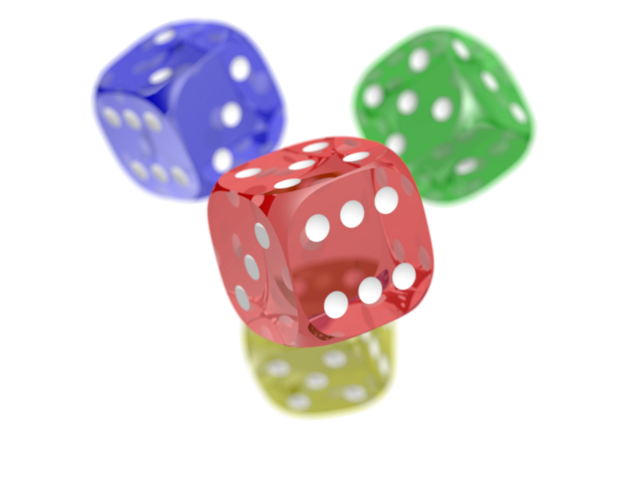
\includegraphics[width=0.7\textwidth]{Figures/example_image.png}
    \caption{Example board configuration solved by the model.}
\end{figure}

\subsection{Results}
Show performance in terms of solution time, and move quality.

\section{Discussion}
\subsection{Limitations}
\begin{itemize}
    \item Model scalability as board complexity increases
    \item Handling dynamic player interaction
\end{itemize}

\subsection{Future Work}
\begin{itemize}
    \item Integration with other AI agents.
    \item Use of reinforcement learning or hybrid approaches.
    \item Implementation of Counting strategies to create a complex probabilistic model. 
\end{itemize}

\section{Conclusion}
We have proposed an integer programming model capable of identifying optimal Rummikub moves from a static game state. This framework serves as a step toward developing intelligent agents capable of playing competitively.

\bibliographystyle{plainnat}
\bibliography{rummikub_research}

\end{document}
